\section{Evaluation}
\label{sec:evaluation}
For evaluation of both models, which are described in section \ref{sec:model}, the tool \textit{Tensorboard} is used. This suite of visualization tools can be used to understand, debug and optimize \textit{TensorFlow} programs. In the context of evaluation, \textit{Tensorboard} is used to visualize the 
\begin{itemize}
	\item accuracy,
	\item loss and
	\item graph
\end{itemize}
of the model. As validation technique the k fold cross validation is being deployed. How this technique works and how it is integrated within the architecture is described in the subsection \ref{subsec:kfoldxvalidation}. In \ref{subsec:experiments} the basic setup used for executing different experiments are explained. The specific results of those experiments for the \textit{SimpleLearningModel} are shown in subsection \ref{subsec:slmexperiment}, while the results yielded by the \textit{OnlyStockLearningModel} are described in the subsection \ref{subsec:onlystockmodelexperiment}. Finally, the results from both models are compared in subsection \ref{subsec:compmodelresults}.

\subsection{K fold cross validation}
\label{subsec:kfoldxvalidation}
The most simple method for cross validation is the \textit{holdout} method. This technique splits the available dataset into two distinct sets - training and validation. In terms of variance this method is disadvantageous as it is not certain which data points end up in the validation set. This can lead to losing important patterns during training and, therefore, underfitting. 
\\
The technique of k fold cross validation provides a method of using the available data efficiently for training as well as validation. The data is split into $k$ subsets and the \textit{holdout} method is applied $k$ times to these sets. In each iteration a different set of the $k$ datasets is used as validation set and the remaining $k-1$ sets are used for training. As a result, each data point is used multiple times for training at some point in the loop and once for validation. Consequently, most of the data is used for fitting so that the bias is greatly reduced and by using most data for validation this also reduces the variance. The swap of training and validation data for each iteration also contributes to the efficiency of this technique. 
\\
The evaluation of the model by the k fold cross validation is achieved by logging the accuracy and loss. Those two scalars are measured for every iteration during the cross validation and after the $k$ iterations for the current epoch. During each of the $k$ iterations the mean of the accuracy and loss for all batches is calculated and written to a \textit{Tensorboard} chart. After the $k$ iterations the mean of all previously calculated average accuracies and losses is determined and also written to a \textit{Tensorboard} chart, whereas the x-axis displays the epoch of this result. The calculation for those mean values is done outside the \textit{TensorFlow} graph. Although this is not best practice, the mean calculation for those scalars would have been quite challenging to do inside the graph as a definition for the epoch is not possible at the level of graph definition. 

\subsection{Experiments for evaluation}
\label{subsec:experiments}
For the validation of the model implementation experiments are executed for both defined models, which are described in detail in subsection \ref{subsec:simplelearningmodel} and \ref{subsec:onlystockmodelexperiment}. The following parameters are varied for a different setup: 
\begin{itemize}
	\item dropout probability, 
	\item hidden size of the LSTM cell, 
	\item learning rate of the optimizer, 
	\item count of folds for cross validation $k$, 
	\item and the number of epochs
\end{itemize}
The mean accuracy and loss after each k fold cross validation as well as the mean overall accuracy and loss are being used as metrics for the rating of parameter configuration. These scalars are logged as described in the previous subsection \ref{subsec:kfoldxvalidation}. 
\\
Overall, four different settings of those parameters are used, wherefore four experiments for each model type are executed. In table \ref{tbl:experiments} these configurations are depicted. 
\renewcommand{\arraystretch}{1.5}
\begin{table}[!ht]
	\begin{center}
		\begin{tabular}{c|c|c|c|c|}
			\multirow{2}{1cm}{} & \multicolumn{4}{c|}{\textbf{Experiment setups}} \\
			 & \textbf{1} & \textbf{2} & \textbf{3} & \textbf{4}\\
			\hline
			\textbf{Hidden size} & 100 &  100 & 200 & 100 \\
			\hline
			\textbf{Dropout probability} & 0.3 & 0.0 & 0.3 & 0.3 \\
			\hline
			\textbf{Learning rate} & 1.0 & 1.0 & 2.0 & 0.5 \\
			\hline
			\textbf{Number of folds k} & 10 & 10 & 10 & 10 \\
			\hline
			\textbf{Number of epochs} & 650 & 650 & 650 & 650 \\
		\end{tabular}
	\end{center}
	\caption{The configurations for all experiments. }
	\label{tbl:experiments}
\end{table}
While the number of folds k for the cross validation as well as the number of epochs for training remain the same for all experiments, the other three parameters are varied. According to a scientific paper about dropout from the university of Toronto (\cite{Srivastava:2014:DSW:2627435.2670313}) the minimal classification error is achieved for a fixed dropout probability $p$ in the range $0.3 \le p \le 0.8$. Therefore, the experiments using dropout are executed with a minimal dropout probability $p = 0.3$. To examine the effects of the hidden size of the LSTM cell and the learning rate of the optimizer on the accuracy and loss, these parameters are also varied. 
\\
Additionally, the trained model is used to predict the rising or falling of stocks unused during the training process. This prediction process is executed ten times and the maximum, minimum and average accuracy for the predictions are logged. Thus conclusions can be made about the applicability of the models for stock prediction. 

\subsection{SimpleLearningModel results}
\label{subsec:slmexperiment}	
The visualized experiment results of the \textit{SimpleLearningModel} are extracted from \textit{Tensorboard}. Within the visualization suite the accuracy and the loss of all experiments were grouped within one graph for better comparability. In figure \ref{fig:acc650epochs} the accuracy over 650 epochs are depicted. 
\begin{figure}[!ht]
	\caption{The mean accuracy of all experiments over 650 epochs of the k fold cross validation with $k=10$. }
	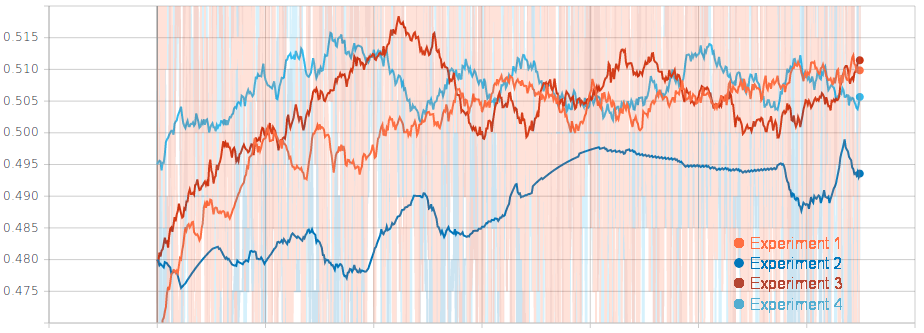
\includegraphics[width=0.95\linewidth]{images/evaluation/slm-k-accuracy.png}
	\label{fig:acc650epochs}
\end{figure}
\\ As expected, the experiment without dropout achieved the lowest accuracy of all experiments. While the other three experiments achieved quite similar results concerning the accuracy, experiment 2 needed about twice the time for the same number of epochs than experiment 1 and 4 with about 22 minutes. This is due to the doubled size of the hidden units, wherefore this setting is unsuitable for training and, also, strongly influences the extent of the loss which can be seen in figure \ref{fig:loss650epochs}. 
\begin{figure}[!ht]
	\caption{The mean loss of all experiments over 650 epochs of the k fold cross validation with $k=10$. }
	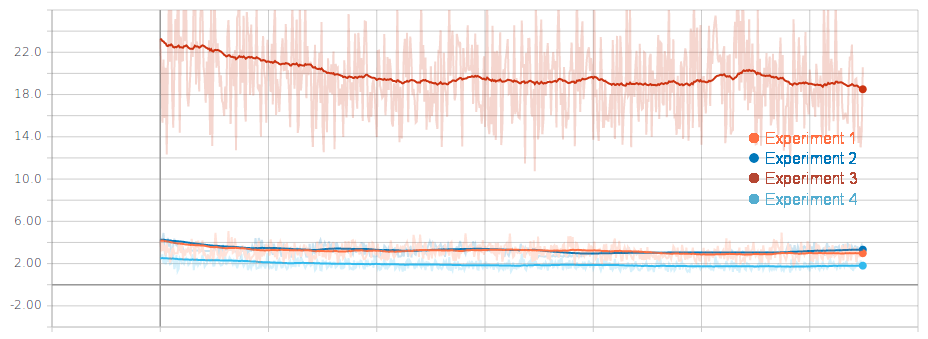
\includegraphics[width=0.95\linewidth]{images/evaluation/slm-k-losses.png}
	\label{fig:loss650epochs}
\end{figure}
\\ Therefore, only experiment 1 and 4 yield acceptable results. In comparison, the accuracy graph of experiment 4 is overall higher than the accuracy graph of experiment 1. This implies that the configuration of experiment 4 is better than the settings of experiment 1. However, regarding the prediction results for a dataset unknown to the trained models, experiment 1 seems to work better. In table \ref{tbl:slmpredictresults} these prediction results are presented. 
\begin{table}[!ht]
	\begin{center}
		\begin{tabular}{c|c|c|c|c|}
			\multirow{2}{1cm}{} & \multicolumn{4}{c|}{\textbf{Experiment prediction results}} \\
			& \textbf{1} & \textbf{2} & \textbf{3} & \textbf{4}\\
			\hline
			\textbf{Minimum} & 50.00 & 43.75 & 43.75 & 31.25 \\
			\hline
			\textbf{Maximum} & 68.75 & 43.75 & 68.75 & 68.75 \\
			\hline
			\textbf{Average} & 61.25 & 43.75 & 50.00 & 51.25 \\
		\end{tabular}
	\end{center}
	\caption{The minimum, maximum and average prediction accuracy in \% of ten predictions for a dataset unknown to the trained \textit{SimpleLearningModel}. }
	\label{tbl:slmpredictresults}
\end{table}
As described in the previous section \ref{subsec:experiments}, these results are collected by using a dataset unknown to the trained models and executing the prediction function ten times. For this validation the settings of experiment 1 achieve a 10\% higher accuracy than the model of experiment 4. The smaller learning rate of experiment 4 in combination with the presented results could imply that this model needs more epochs to converge to the optimum. However, the losses of all experiments quickly converge to a minimum. In figure \ref{fig:loss650epochs2} the graph of the third experiment is removed due to its magnitude so that a more precise view of the remaining loss graphs can be seen. 
\begin{figure}[!ht]
	\caption{The mean loss of the experiments 1, 2 and 4 over 650 epochs of the k fold cross validation with $k=10$. }
	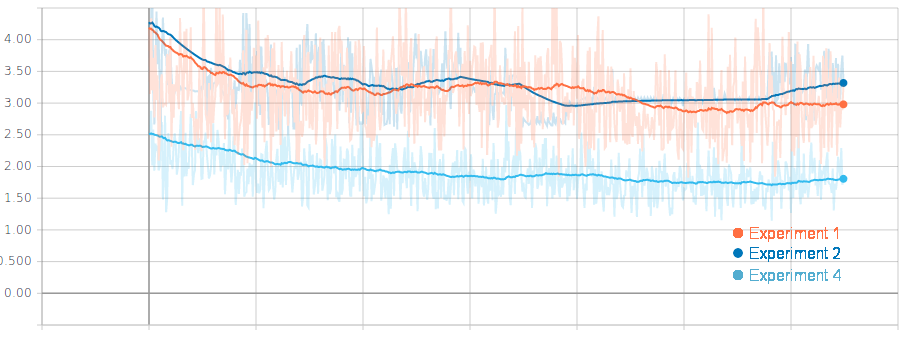
\includegraphics[width=0.95\linewidth]{images/evaluation/slm-k-losses-2.png}
	\label{fig:loss650epochs2}
\end{figure}

\subsection{OnlyStockLearningModel results}
\label{subsec:onlystockmodelexperiment}
In figure \ref{fig:OSLM_k-accuracy} you can see the accuracy of the four experiments described in table \ref{tbl:experiments}. The loss can be seen in figure \ref{fig:OSLM_k-loss}. The model without using dropout (experiment 2) performed best. This seems to be reasonable because if the dropout drops the only input, like in the other three experiments, the model can not use any data for learning. The model with the biggest hidden size (experiment 3) is not performing better than the other models and therefore it does not make sense to increase the hidden size. The model of experiment 4 has the lowest learning rate and therefore it should be possible for it to find a better minimum. But as the accuracy shows there is a great variance and the accuracy is not converging against any value.\\
\begin{figure}[tb]
	\caption{A Graph depicting the mean accuracy of the OnlyStockLearningModel over 650 epochs of the k fold cross validation with $k=10$. The orange line shows the accuracy during training for experiment 1. Its mean accuracy is about $49\%$. The dark blue graph is presenting the results of the second experiment. It has the best mean accuracy of about $52\%$. The red line showing experiment 3 has about the same mean accuracy as the forth experiment (light blue line). The mean accuracy is at about $48\%$ accuracy.}
	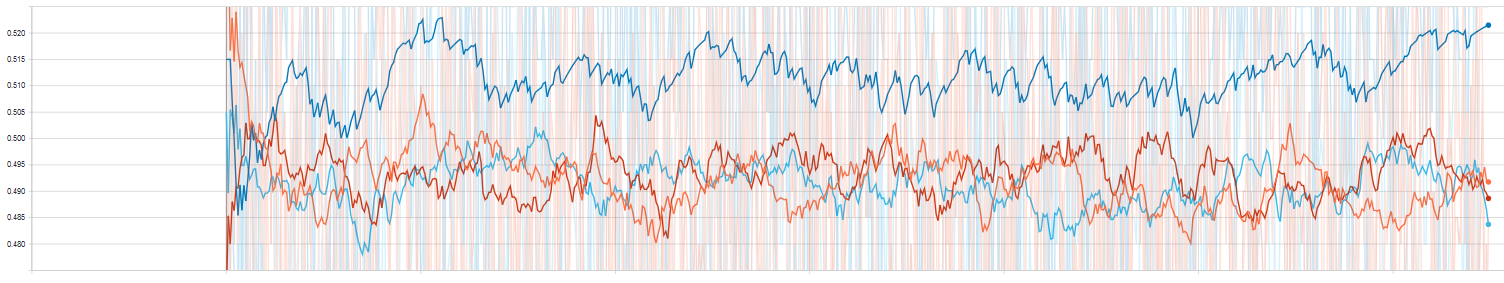
\includegraphics[width=0.95\linewidth]{images/OSLM_k-accuracy.PNG}
	\label{fig:OSLM_k-accuracy}
\end{figure}
\begin{figure}[tb]
	\caption{A Graph depicting the mean loss of the OnlyStockLearningModel over 650 epochs of the k fold cross validation with $k=10$. The orange line depicts the loss of the first experiment. It has nearly the same mean loss of about $4.7$ as the second experiment (dark blue line). Experiment 3 has a much higher loss, depicted with the red line, of about $24.6$. The loss of experiment 4 is shown in the light blue line. Its mean value is the lowest with about $1.4$.}
	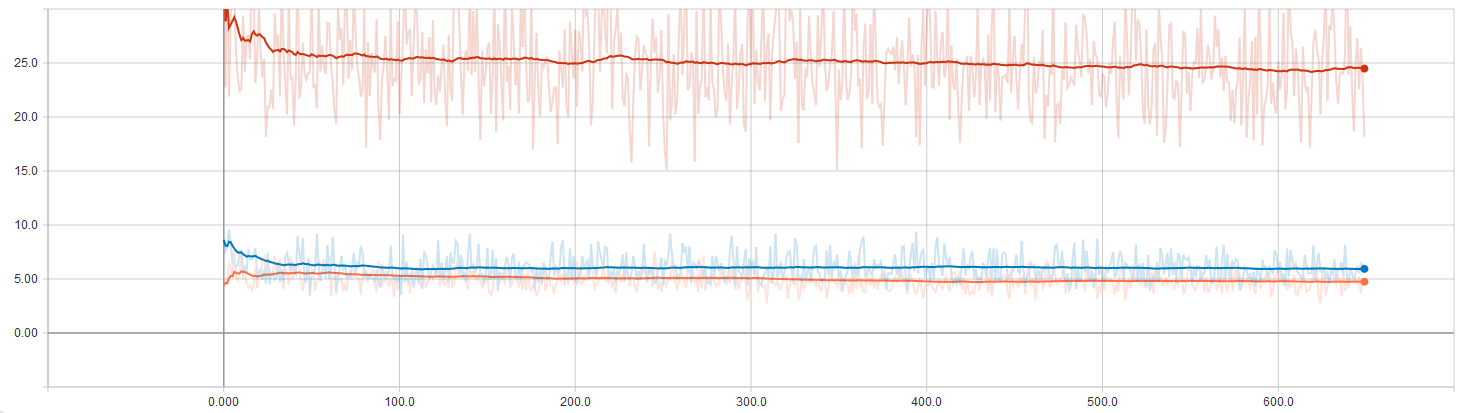
\includegraphics[width=0.95\linewidth]{images/OSLM_k-loss.PNG}
	\label{fig:OSLM_k-loss}
\end{figure}
In table \ref{tbl:oslmpredictresults} you can see how the models performed on data not seen during training. The test dataset contains only 16 entries, so the results have to be watched carefully.
\begin{table}[!ht]
	\begin{center}
		\begin{tabular}{c|c|c|c|c|}
			\multirow{2}{1cm}{} & \multicolumn{4}{c|}{\textbf{Experiment prediction results}} \\
			& \textbf{1} & \textbf{2} & \textbf{3} & \textbf{4}\\
			\hline
			\textbf{Minimum} & 50.00 & 50.00 & 37.50 & 37.50 \\
			\hline
			\textbf{Maximum} & 56.25 & 50.00 & 56,25 & 62.50 \\
			\hline
			\textbf{Average} & 53.63 & 50.00 & 46.88 & 50.00 \\
		\end{tabular}
	\end{center}
	\caption{The minimum, maximum and average prediction accuracy in \% of ten predictions for a dataset unknown to the trained \textit{OnlyStockLearningModel}. }
	\label{tbl:oslmpredictresults}
\end{table}
The model without using dropout (experiment 2) has a lower accuracy on unseen data than it had during training, whereas the model of the first experiment is even better on this test data. The forth model has like during training the biggest variance and is performing equally well as the second model. The third model, although it has the biggest hidden size and can store the most information, has the lowest accuracy on unseen data. All four models do not have an accuracy during training and testing which is good enough to make me belief that they can predict the trend of a stock better than an financial expert could do.


\subsection{Comparison of model results}
\label{subsec:compmodelresults}	
Comparing the results of the SimpleLearningModel \ref{subsec:slmexperiment} with the results of the OnlyStockLearningModel \ref{subsec:onlystockmodelexperiment} can help us to decide whether the data from google trends is useful in predicting the stock course.\\
First of all we want to compare the differences between the two models according to the changes made to the configuration. As already mentioned in subsection \ref{subsec:onlystockmodelexperiment} dropout does not help the OnlyStockLearningModel, whereas the SimpleLearningModel improves with using dropout. Varying the hidden size of the LSTM cell does not lead to an improvement neither in the SimpleLearningModel nor in the OnlyStockLearningModel. The same can be said about the reduction of the learning rate.\\
During training the second experiment with the OnlyStockLearningModel had the best accuracy, but on unseen data it is slightly worse than nearly all experiments (expect experiment 2) with the SimpleLearningModel. On unseen data the first experiment of the SimpleLearningModel has by far the best accuracy with $61.25\%$. But this has to be watched carefully because of the small number of samples in the test dataset.\\
There is only a small variance of the accuracy in all experiments during training. The loss is also changing very slowly after about epoch $150$. In contrast the variance during testing is really high especially for the forth experiment of both models.\\
If we consider the results of the first experiment of both models as a spike because they have the best average accuracy on unseen data, the three other experiments leaded to nearly the same results for both models. As a consequence the data from google trend does not really help to predict the stock course.

